\documentclass{standalone}

\usepackage{pgfplots,tikz,amsmath,amssymb}
\begin{document}
    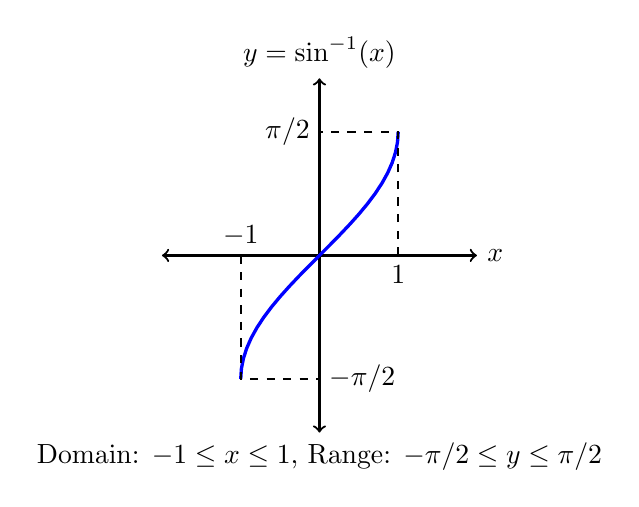
\begin{tikzpicture}
        \draw[thick, <->] (-2,0) -- (2,0) node[anchor=west]{$x$};
        \draw[thick, <->] (0,-2.25) -- (0,2.25) node[anchor=south]{$y=\sin^{-1}(x)$};
        \draw[color=blue, very thick, domain=-1.57:1.57] plot ({sin(deg(\x))},{\x});
        \draw (1,0) node[anchor=north]{$1$};
        \draw (-1,0) node[anchor=south]{$-1$};
        \draw (0,1.57) node[anchor=east]{$\pi/2$};
        \draw (0,-1.57) node[anchor=west]{$-\pi/2$};
        \draw[thick, dashed] (1,0) -- (1,1.57) -- (0,1.57);
        \draw[thick, dashed] (-1,0) -- (-1,-1.57) -- (0,-1.57);
        \draw (0,-2.25) node[anchor=north]{Domain: $-1\le x \le 1$, Range: $-\pi/2 \le y
        \le \pi/2$};
    \end{tikzpicture}
    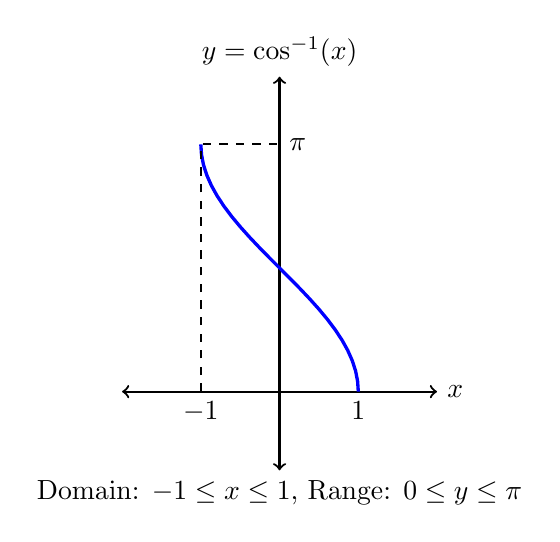
\begin{tikzpicture}
        \draw[thick, <->] (-2,0) -- (2,0) node[anchor=west]{$x$};
        \draw[thick, <->] (0,-1) -- (0,4) node[anchor=south]{$y=\cos^{-1}(x)$};
        \draw[color=blue, very thick, domain=0:3.14] plot ({cos(deg(\x))},{\x});
        \draw (1,0) node[anchor=north]{$1$};
        \draw (-1,0) node[anchor=north]{$-1$};
        \draw (0,3.14) node[anchor=west]{$\pi$};
        \draw[thick, dashed] (-1,0) -- (-1,3.14) -- (0,3.14);
        \draw (0,-1) node[anchor=north]{Domain: $-1\le x \le 1$, Range: $0 \le y
        \le \pi$};
    \end{tikzpicture}
    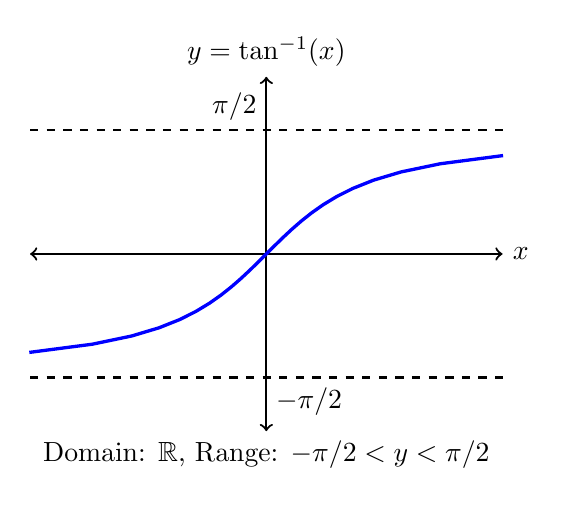
\begin{tikzpicture}
        \draw[thick, <->] (-3,0) -- (3,0) node[anchor=west]{$x$};
        \draw[thick, <->] (0,-2.25) -- (0,2.25) node[anchor=south]{$y=\tan^{-1}(x)$};
        \draw[color=blue, very thick, domain=-1.25:1.25] plot ({tan(deg(\x))},{\x});
        \draw (0,1.57) node[anchor=south east]{$\pi/2$};
        \draw (0,-1.57) node[anchor=north west]{$-\pi/2$};
        \draw[thick, dashed] (-3,1.57) -- (3,1.57);
        \draw[thick, dashed] (-3,-1.57) -- (3,-1.57);
        \draw (0,-2.25) node[anchor=north]{Domain: $\mathbb{R}$, Range: $-\pi/2 < y
        < \pi/2$};
    \end{tikzpicture}
\end{document}
